\chapter{Opis projektnog zadatka}


Cilj ovog projekta je razvoj programske potpore za stvaranje web aplikacije \textit{"Pomozi mi"} koja svojim korisnicima omogućuje potraživanje nečije pomoći, ali i pružanje vlastite pomoći. 
Primjerice, tako bi korisnik mogao otići po mlijeko za bolesnu susjedu koja je to zatražila, a ujedno nekoga iz IT sektora zamoliti da mu pomogne namjestiti postavke pisača. 

Pretragom tržišta trenutno dostupnih aplikacija, nismo pronašli aplikaciju koja nudi slična rješenja. Većina pronađenih aplikacija nudi vrlo specifičan način pomoći, a aplikacije su isključivo za Android i iOS mobilne uređaje \textit{(Be my eyes, Kindly, uCiC, Mayo)}. Najsličnija aplikacija našem rješenju je \textit{Mayo (u razvoju, slika 2.1)}, ali i tu su vidljive velike razlike kao što su: registracija u spomenutu aplikaciju nije potrebna (anonimnost) te dostupnost samo za mobilne uređaje.\\


\begin{figure}[H]
	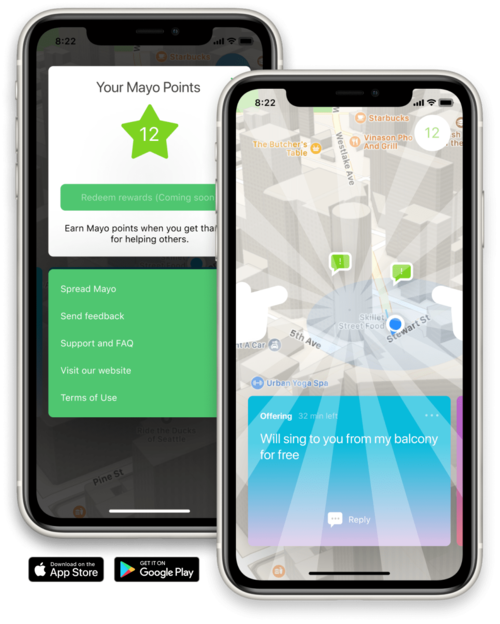
\includegraphics[scale=0.2]{slike/mayo-hero.PNG} %veličina slike u odnosu na originalnu datoteku i pozicija slike
	\centering
	\caption{Primjer konkurentne aplikacije}
\end{figure}

Zbog prirode naše aplikacije, samo će korisnici s napravljenim računom moći pregledati zahtjeve za pomoć i objaviti svoje.

\pagebreak
 Da bi korisnik napravio svoj korisnički račun, bit će potrebni:

\begin{packed_item}
	\item Korisničko ime
	\item E-mail adresa
	\item Zaporka
	\item Ime
	\item Prezime
	\item Preferirana lokacija
	\item Kontakt broj mobitela
\end{packed_item}

Kada korisnik stvori svoj račun, omogućena mu je prijava u aplikaciju unosom svojeg korisničkog imena i zaporke.

Prijavljenom korisniku sada se prikazuju zahtjevi za pomoć na početnom zaslonu, a pomoću intuitivnog korisničkog sučelja može postaviti svoj zahtjev za koji potražuje pomoć.

Opišimo sada kako će tipični korisnik navigirati našom aplikacijom.
Kada korisnik želi pomoći, odabire zahtjev s liste svih aktivnih zahtjeva
koji se nalaze unutar jednog kilometra od lokacije uređaja. Lista se može
proširiti na veće geografsko područje. Korisnik koji će provesti odabrani zahtjev
se smatra \textbf{izvršiteljem zahtjeva}. Valja napomenuti kako je svaka lista sortirana po određenom redoslijedu i omogućeno je
filtriranje zahtjeva prema kategorijama. Primjerice, moguće je gledati virtualne ili zahtjeve s lokacijom.
Kada korisnik traži pomoć, govorimo o ulozi \textbf{autora zahtjeva}. Prilikom zadavanja, autor unosi opis i kontakt podatke poput broja mobitela, adrese (opcionalno) i datum i/ili vrijeme do kada se zahtjev treba izvršiti (opcionalno).
Budući da se više mogućih izvršitelja može javiti na jedan zahtjev, odabir konačnog vrši se metodom trostrukog rukovanja. To ćemo najbolje razjasniti primjerom: 

	\begin{packed_item}
	\item \textit {Teta Marica želi da joj netko donese 3kg krumpira (autor zahtjeva).}
	
	\item \textit {Ante i Marko vide da teta Marica treba pomoć i jave se na zahtjev (mogući izvršitelji).}
	\item \textit {Marica vidi da su se obojica javila, ali je Ante bolji izvršitelj i njega odabere (Ante je izvršitelj).}
	\end{packed_item}
	Kada je izvršitelj odabran, razmjenjuju se kontakt informacije i kreće proces izvršenja koji ostavljamo gore navedenim dionicima. 
	
	Postavlja se pitanje kako je teta Marica znala da je Ante "bolji" izvršitelj? Zahvaljujući sustavu međusobnog ocjenjivanja korisnika! Po izvršenju zahtjeva autor označava da je zahtjev izvršen nakon čega se korisnici međusobno ocjenjuju ocjenama od 1-5 te opcionalno upisuju komentare. Kako novi korisnici ne bi ostali zakinuti za povjerenje budućih autora zahtjeva, ocjenjivanje bilo kojeg korisnika aplikacije moguće je u bilo kojem trenutku (ne samo nakon izvršenja zadatka) i ocjene se vide u detaljima profila, kao i komentari. Također, moguće je vidjeti i
	"lance povjerenja": da je korisnik kojeg ste vi visoko ocijenili ocijenio korisnika
	čiji profil gledate.
	
	Kako bi se čovjek mogao prisjetiti svoje i tuđe humanosti, svaki korisnik može vidjeti listu zahtjeva koje je zadao i izvršio. Sustav
	omogućuje i dodatne izvještaje/preglede, posebno one koji omogućuju
	prikaz najboljeg pomagača u tekućoj godini.
	
	Da bismo zajednicu učinili sigurnijom, uveli smo ulogu \textbf{administratora}. Administratori se brinu oko sadržaja koji se objavljuje. Imaju ovlasti
	brisanja zahtjeva koji se smatra opasnim, nemogućim, lažnim ili neetičkim te
	privremenog i trajnog blokiranja korisnika aplikacije. Administratori se
	dodjeljuju prema geografskim lokacijama. 
	
	Na kraju ovog opisa treba spomenuti nekoliko posebnosti. Ukoliko korisnik tijekom zadavanja zahtjeva ne želi unijeti lokaciju, taj zahtjev će se prikazivati svim korisnicima neovisno o njihovoj lokaciji. Sjetimo se čovjeka koji je tražio pomoć oko namještanja postavki pisača, taj zahtjev je razumno označiti kao virtualni.
	Također, kako naša spomenuta teta Marica ne bi morala uvijek unositi adresu kada stvara novi zahtjev, adresa zahtjeva može se povući iz adrese s kojom je registrirana i tako Marici uštedjeti nekoliko sekundi svakim zahtjevom.
\eject


